\chapter{Marco de Referencia}

Se define como el basamento teórico y experimental. Este ayuda a entender mejor el problema, la metodología y la solución

\section{Antecedentes}
    \begin{sectext}
        Los antecedentes pueden desprenderse en 2 tipos:

        \begin{itemize}
            \item \textbf{Antecedentes del problema:} ¿Desde cuándo está presente tu problema?
            \item \textbf{Antecedentes de la investigación:} ¿Quiénes otros han estudiado ese problema?
        \end{itemize}

        % \newline 
        
        En la sección de antecedentes de las tesis nos referimos a los antecedentes de investigación. (Otros trabajos que ya han sido realizados). Estos tienen relación con el tema: Variables dependiente, independiente u la metodología.

        \begin{figure}[H]
            \centering
            %\isPreprints{\centering}{} % Only used for preprints
            \caption{Cantidad de Antecedentes necesarios. 
            \label{fig-cantidad-antecedentes}}    
                
            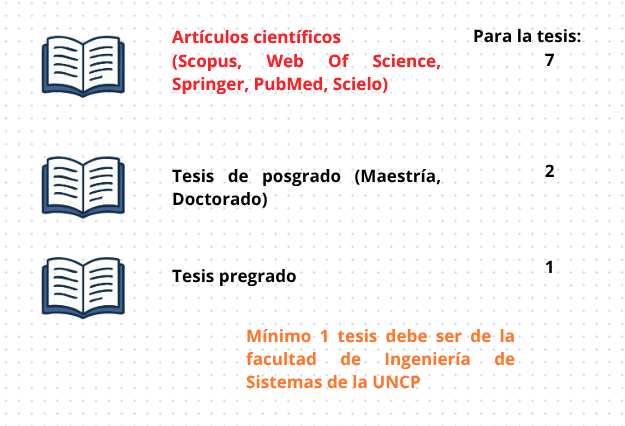
\includegraphics[width=10.0 cm]{src/imgs/cant-antecedentes.png}

            \vspace{0.1cm}
            \small Elaborado a partir de ...
        \end{figure}

        \begin{figure}[H]
            \centering
            %\isPreprints{\centering}{} % Only used for preprints
            \caption{Estructura de redacción de los antecedentes.
            \label{fig-estructura-antecedentes}}    
                
            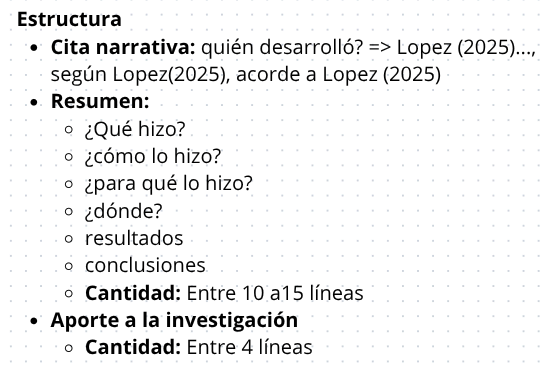
\includegraphics[width=10.0 cm]{src/imgs/estructura-antecedentes.png}

            \vspace{0.1cm}
            \small Elaborado a partir de ...
        \end{figure}

        \textcite{arensmeyer_system_2024}, describieron un novedoso sistema de planificación quirúrgica tridimensional en tiempo real basado en realidad mixta mediante el uso de un visor con tecnología de transmisión de video (video pass-through) y el renderizado volumétrico de datos de tomografía computarizada (TC). La investigación tuvo como finalidad mejorar la evaluación preprocedural y la planificación de tratamientos personalizados en cirugías complejas de la cavidad torácica, minimizando la necesidad de guías basadas en radiación intraoperatoria. Para validar el concepto, los autores aplicaron el sistema clínico en el Hospital Universitario de Bonn (Alemania), proyectando y alineando hologramas anatómicos interactivos sobre los cuerpos de tres pacientes oncológicos masculinos atendidos entre 2022 y 2023. Como principales resultados, los cirujanos lograron identificar con precisión las regiones de interés y distinguir la relación geométrica entre las lesiones y las estructuras blandas u óseas adyacentes utilizando herramientas de manipulación de imagen e integración de sensores LiDAR. Los autores concluyeron que el uso de superposiciones holográficas en entornos de realidad extendida resulta altamente prometedor para optimizar el abordaje de operaciones torácicas complejas o menos estandarizadas, proporcionando una perspectiva quirúrgica superior en comparación con las imágenes bidimensionales convencionales. El trabajo de \textcite{arensmeyer_system_2024} resalta el problema identificado por la presente investigación, aseverando que la poca utilización de las imágenes reconstruidas en 3D para la planificación quirúrgica de cirugías torácicas, los cuales al ser combinados con métodos inmercivos como la realidad Virtual u Mixta mejoran la precisión en la planificación. \newline
        
        \textcite{bakhuis_essential_2023} investigaron el valor clínico añadido de la tecnología de realidad virtual (RV) en el planeamiento preoperatorio de segmentectomías pulmonares. La investigación tuvo como finalidad evaluar la cantidad de modificaciones críticas en los planes quirúrgicos tradicionales y analizar la planificación preoperatoria ante una mejor perspectiva espacial de la anatomía broncovascular del paciente. El estudio se realizó con un equipo de tres cirujanos y un residente del Centro Médico de la Universidad de Erasmus en Rotterdam (Países Bajos); por su parte, se analizaron los resultados de 50 pacientes programados para resección segmental sublobar entre junio de 2020 y septiembre de 2021. El desarrollo metodologógico constó del procesamiento de las tomografías computarizadas (TC) convencionales mediante inteligencia artificial con la plataforma PulmoVR para realizar segmentaciones automáticas de los bordes pulmonares y vasos anatómicos. Como principales resultados, la visualización inmersiva en 3D provocó que los cirujanos modificaran el plan quirúrgico original en el 52\% de los casos (debido a localizaciones tumorales erróneas o variantes anatómicas ocultas), logrando una tasa de éxito de resección radical confirmada del 98\%. Los autores concluyeron que la integración de la realidad virtual preoperatoria proporciona una comprensión anatómica superior y personalizada, permitiendo realizar cirugías con mayor preservación de tejido pulmonar sano sin comprometer la radicalidad oncológica. El trabajo de \textcite{bakhuis_essential_2023} responde directamente a la problemática establecida por el presente trabajo respecto a la limitada imagen mental que los cirujanos son capaces de percibir respecto a la patología y anatomía del paciente solo mediante el uso de imágenes médicas en el marco bidimensional. \newline
    \end{sectext}
    

\section{Marco Teórico}
    \begin{sectext}
        Define hasta qué punto se enmarca la investigación.

        Como recomendación, no debes poner más conceptos de los que usarás. Ya que de lo contrario se custionará el: ¿Y dónde utilizó tal u tal concepto?

        Aquí de cierta manera se delimita el alcance. Míralo como los márgenes de un estadio de fútbol.

        \subsection{Concepto como subsección 1}
            \begin{subsectext}
                Lorem ipsum dolor sit amet consectetur adipisicing elit. Voluptate dolor sapiente accusamus vel tempore distinctio dicta architecto at beatae aliquam, cumque consequatur iure, aspernatur unde ratione a enim non molestiae voluptas nemo. Enim sed laudantium repellat odit eligendi quam facilis perspiciatis similique quo impedit praesentium eos error et corrupti quidem, aperiam consequuntur debitis libero tempora commodi aut voluptatum? Quasi numquam temporibus, tempore amet commodi tempora, mollitia hic esse molestias earum eligendi, sint rem suscipit! Quia est veritatis aspernatur nihil, eius consectetur tenetur quaerat, sunt quo numquam nesciunt ipsam iure reiciendis quisquam facilis totam obcaecati rem, culpa praesentium voluptates voluptatum sit. 

                \begin{itemize}
                    \item \textbf{Item 1}\newline
                    Lorem ipsum dolor sit amet consectetur adipisicing elit. Voluptate dolor sapiente accusamus vel tempore distinctio dicta architecto at beatae aliquam, cumque consequatur iure, aspernatur unde ratione a enim non molestiae voluptas nemo. 

                    \item \textbf{Item 2}\newline
                    Lorem ipsum dolor sit amet consectetur adipisicing elit. Voluptate dolor sapiente accusamus vel tempore distinctio dicta architecto at beatae aliquam, cumque consequatur iure, aspernatur unde ratione a enim non molestiae voluptas nemo.
                \end{itemize}
            \end{subsectext}

        \subsection{Concepto como subsección 2}
            \begin{subsectext}
                Lorem ipsum dolor sit amet consectetur adipisicing elit. Voluptate dolor sapiente accusamus vel tempore distinctio dicta architecto at beatae aliquam, cumque consequatur iure, aspernatur unde ratione a enim non molestiae voluptas nemo. Enim sed laudantium repellat odit eligendi quam facilis perspiciatis similique quo impedit praesentium eos error et corrupti quidem, aperiam consequuntur debitis libero tempora commodi aut voluptatum? Quasi numquam temporibus, tempore amet commodi tempora, mollitia hic esse molestias earum eligendi, sint rem suscipit! Quia est veritatis aspernatur nihil, eius consectetur tenetur quaerat, sunt quo numquam nesciunt ipsam iure reiciendis quisquam facilis totam obcaecati rem, culpa praesentium voluptates voluptatum sit. 

                \begin{itemize}
                    \item \textbf{Item 1}\newline
                    Lorem ipsum dolor sit amet consectetur adipisicing elit. Voluptate dolor sapiente accusamus vel tempore distinctio dicta architecto at beatae aliquam, cumque consequatur iure, aspernatur unde ratione a enim non molestiae voluptas nemo. 

                    \item \textbf{Item 2}\newline
                    Lorem ipsum dolor sit amet consectetur adipisicing elit. Voluptate dolor sapiente accusamus vel tempore distinctio dicta architecto at beatae aliquam, cumque consequatur iure, aspernatur unde ratione a enim non molestiae voluptas nemo.
                \end{itemize}

            \end{subsectext}
    \end{sectext}

\section{Modelo Aplicativo}
    \begin{sectext}
        Delimita el paso del modelo teórico al modelo aplicativo (de la teoría a la realidad)

        Flujograma desde el cual el tesista lleva toda la teoría a la práctica. Esto a través de una serie de pasos estructurados.

        \begin{figure}[H]
            \centering
            %\isPreprints{\centering}{} % Only used for preprints
            \caption{Estructura del modelo aplicativo.
            \label{fig-estructura-antecedentes}}    
                
            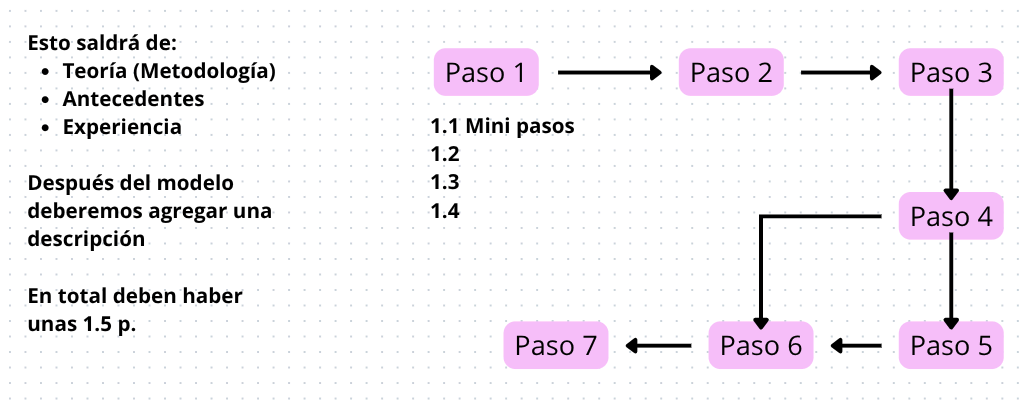
\includegraphics[width=10.0 cm]{src/imgs/modelo-aplicativo.png}

            \vspace{0.1cm}
            % \small EN CASO DE SER BAJO ELABORACIÓN PROPIA, NO HACE FALTA AGREGAR LA NOTA
        \end{figure}

    \end{sectext}

\section{Marco Conceptual}
    \begin{sectext}
        Es un glosario u diccionario en el cual incluimos los términos que necesitamos definir, pero que no son tan relevantes como para considerar en el marco teórico. De preferencia siempre usar citas parentéticas.

        Debemos considerar entre 15 a 20 términos. y cada definición debe tener de entre 2 a 3 líneas. Los términos no deben estar enumerados, pero sí ordenados alfabéticamente.

        \begin{itemize}
        \item \textbf{Conflicto de Vergencia-Acomodación (VAC)}: Contradicción fisiológica que causa fatiga visual cuando los ojos convergen en un objeto 3D virtual pero deben enfocar físicamente (acomodación) a la distancia fija de una pantalla 2D convencional \parencite{blundell_uncertain_2017}.

        \item \textbf{Pantallas de volumen barrido (Swept-volume)}: Dispositivos volumétricos que crean el espacio de visualización mediante el movimiento mecánico rápido y cíclico (ya sea rotacional o de traslación) de una superficie de proyección \parencite{blundell_classification_2002}.
        
        \item \textbf{Technology Readiness Level (TRL)}: Escala de nueve niveles creada inicialmente por la NASA para evaluar la madurez, el riesgo y el avance de una nueva tecnología desde su concepción hasta su despliegue operativo \parencite{salazar_zegarra_taxonomitecnicas_2022}.

        \item \textbf{Vóxel}: Es el equivalente tridimensional de un píxel; consiste en una región o elemento de volumen localizado que emite, refleja o absorbe la luz para conformar una imagen gráfica sólida en el espacio \parencite{blundell_classification_2002}.
        \end{itemize}
    \end{sectext}
